\section{Corpi macchina} \label{sec:analog_corpimacchina}
I produttori e gli appassionati hanno inventato moltissimi corpi macchina, per la più varie necessità.
I più diffusi tuttavia, specialmente quelli che oggi sono più usati tra i fotografi, sono molto simili ai corpi macchina delle fotocamere digitali.

A seguire alcuni tipi di corpi macchina:
\begin{itemize}
    \item[-] \nameref{subsec:slr}
    \item[-] \nameref{subsec:slrmodulari}
    \item[-] \nameref{subsec:telemetro}
    \item[-] \nameref{subsec:tlr}
    \item[-] \nameref{subsec:bancoottico}
\end{itemize}

\subsection{SLR} \label{subsec:slr}
Il funzionamento è esattamente lo stesso delle DSLR, con la differenza principale che dietro la lente c'è una pellicola e non un sensore digitale.

Sul retro della fotocamera non c'è lo schermo, ma c'è un vano, che prende tutta la larghezza della fotocamera; si può aprire per inserire/riprendere, la pellicola.
Questo vano ha due scompartimenti per la pellicola, uno sulla sinistra, uno sulla destra, e al centro va la pellicola stesa, pronta per catturare le immagini.

\begin{figure*}[h]
    \centering
    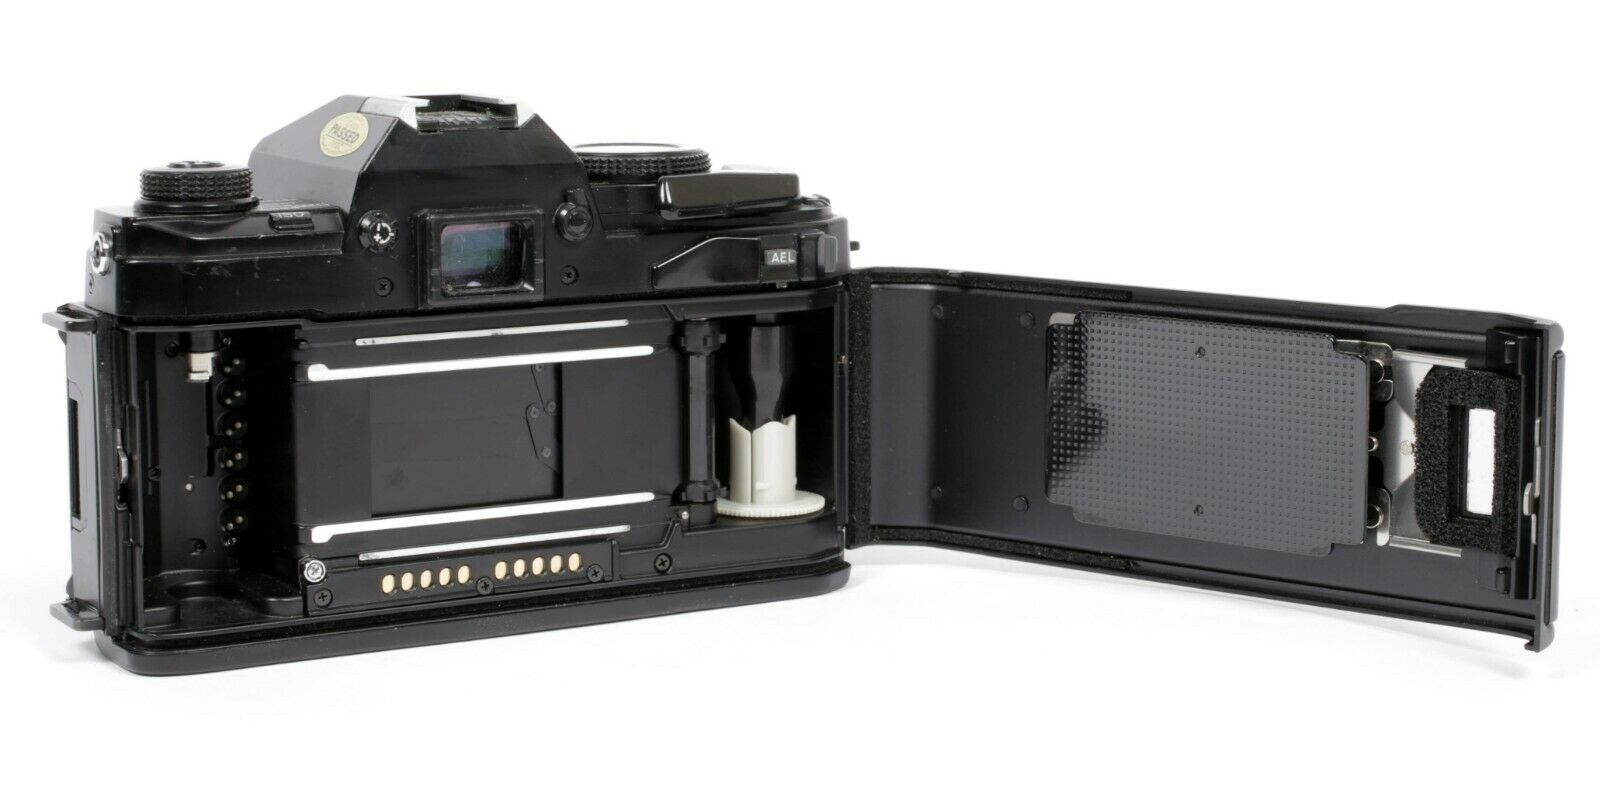
\includegraphics[width=\textwidth]{slr_internet.jpg}
\end{figure*}

Le pellicole sono vendute, in quasi tutti i formati, sottoforma di rotolini, con la pellicola che si avvolge su sé stessa.
Nello scompartimento di sinistra si mette la pellicola, che viene aggancianta al rocchetto a destra.
Ad ogni foto la pellicola deve essere avvolta nel rocchetto sulla destra; quando la pellicola finisce si riavvolge sul rocchetto di sinistra (quello della pellicola) e si riprende la pellicola.

Fotocamere analogiche più tecnologiche hanno un motorino che avvolge la pellicola in modo automatico ad ogni scatto; se questo motorino non c'è bisogna, con una levetta posta sopra la macchinetta, avvolgere la pellicola dopo ogni scatto.
Nella foto di cui sopra la levetta si può vedere a destra del mirino.


\subsection{SLR modulari} \label{subsec:slrmodulari}
Esistono SLR modulari, molto diffuse tra le fotocamere medio formato di fascia alta, come le famose Hasselblad.
Il funzionamento è analogo a quello delle normali SLR, la differenza sta nel modo in cui è fatto il corpo macchina.

Ad oggi la Hasselblad produce fotocamere digitali medio formato, e ancora adotta questo stile modulare, molto iconico.

Il pezzo principale, di forma cubica, contiene il meccanismo a specchi. Sul davanti si monta l'obiettivo. Sul sopra del cubo si monta il mirino, che può essere a pentaprisma (come quello delle SLR) o \textbf{a pozzetto}, che non monta il pentaprisma e permette di vedere l'immagine dall'alto, riflessa direttamente dallo specchio a 45º. Mentre i mirini a pentaprisma montano un piccolo vetrino per osservare la scena, i mirini a pozzetto usano lastrine di vetro smerigliato, e sono pensati per osservare la scena con l'occhio non appoggiato direttamente sul mirino, ma un po' distante.
Sul retro della fotocamera si monta il \textit{dorso}, lo scompartimento dove si carica la pellicola.

Il vantaggio di montare le piccole sul dorso, rimuovibile, è la possibilità di poter cambiare, tra uno scatto e l'altro, la pellicola, per poter fare foto diverse.
Normalmente, sulle fotocamere analogiche, una volta montata la pellicola si praticamente costretti a finire la pellicola prima di poterla cambiare.

Questi corpi macchina sono spesso destinati all'utilizzo in studio, dove si può usare un cavalletto e l'ambiente è più controllato, colpa anche della minore ergonomia.


\subsection{Fotocamera a telemetro} \label{subsec:telemetro}
Sono fotocamere che usano un \textit{telemetro} per la messa a fuoco.

A grandi linee, dal mirino di un telemetro, si vedono due immagini riflesse da due specchi diversi; quando le due immagini coincidono in un punto, allora quel punto è stato messo a fuoco.

Molti modelli di questo tipo di fotocamera non hanno il sistema a specchi di una SLR, sono quasi l'equivalente analogico di una mirrorless.
Notiamo come su pellicola non si può costruire una mirrorless così come la intendiamo con le mirrorless digitali; se rimuoviamo lo specchio non avremmo modo di vedere cosa si sta fotografando.

Soluzione? Il mirino semplicemente non mostra direttamente quello che mostra la fotocamera. Un difetto di questo approccio è che quello che si vede dal mirino è leggermente sfasato rispetto a quello che vede l'obiettivo; chi fotografa deve tenerne conto e adattarsi di conseguenza.


\subsection{Reflex biottica - TLR} \label{subsec:tlr}
Chiamate in inglese anche \textbf{TLR - Twin Lens Reflex}.

Sono fotocamere che si sviluppano in verticale, ed hanno due obiettivi: uno che dà sul sensore, e l'altro che mostra l'inquadratura al fotografo.

L'obiettivo posto in alto è quello usato per inquadrare. La luce rimbalza su uno specchio posto a 45º, ma a differenza delle SLR non c'è il pentaprisma che fa arrivare la luce dietro, bensì usano un \textit{mirino a pozzetto}, che funziona come i mirini a pozzetto montati sulle SLR modulari.

Sono fotocamere, dal punto di vista del funzionamento, più semplici e silenziose delle SLR. Il rovescio della medaglia è che nella quasi totalità dei modelli le lenti non sono interscambiabili, non sono disponibili lenti zoom, e siccome la lente superiore (i.e. quella usata per inquadrare) non ha il diaframma, non è possibile vedere in anticipo come sarà la profondità di campo della foto.

Molte fotocamere biottica sono medio formato, e ad oggi sono un buon modo per approcciarsi alla fotografia analogica su medio formato con prezzi contenuti.


\subsection{Banco ottico} \label{subsec:bancoottico}
Sono fotocamere grandi e pesanti che si usano per fare foto su pellicole grande formato. Sono una versione sotto steroidi delle fotocamere a soffietto.

Sono stati fra i primi corpi macchina. Corpi macchina di questo tipo, nell'Ottocento, insieme al resto dell'attrezzatura, potevano superare i 200kg di peso, rendendo un lavoro non poco faticoso il trasporto dell'attrezzatura fotografica.
I fotografi di montagna che volevano fare qualche scatto erano costretti ad assumere persone che aiutassero con il trasporto.

Oggi il peso è certamente diminuito, grazie anche ai diversi materiali usati, ma le fotocamere restano comunque ingombranti e pesanti rispetto alle altre tipologie di fotocamera.
Per questo e per altri motivi, fotocamere di questo tipo sono esclusivamente usate su treppiedi fissi al terreno.

Poiché l'obiettivo è vincolato al retro della fotocamera dal soffietto, questo fotocamere permettono spesso di poter decentrare e basculare (vedi \nameref{subsec:lentidecentrabili}) la lente.

L'inquadratura si vede dal retro della fotocamera, su una grande lastra di vetro smerigliato. Notiamo che queste fotocamere sono una versione evoluta delle camere oscure, e che quindi l'immagine è capovolta sul vetro smerigliato.

Sia a causa delle dimensioni, che dei costi e dei tempi per una singola foto, queste le pellicole per grande formato non sono vendute in rotoli, come per le pellicole 135 e 120.
Si vendono singoli fogli di pellicola, che sono montati sulla fotocamera grazie ad un supporto specifico.

Le preparazione per una singola foto può richiedere diversi minuti, e un singolo foglio (i.e. una singola foto) può costare 2$\euro$ o più, senza contare il successivo costo (sia in termini di denaro che di tempo) per \textit{sviluppare} la pellicola e stamparla.